\chapter{Theoretical Foundation}
\label{sec:theory}


\begin{figure}[ht]
  \centering
  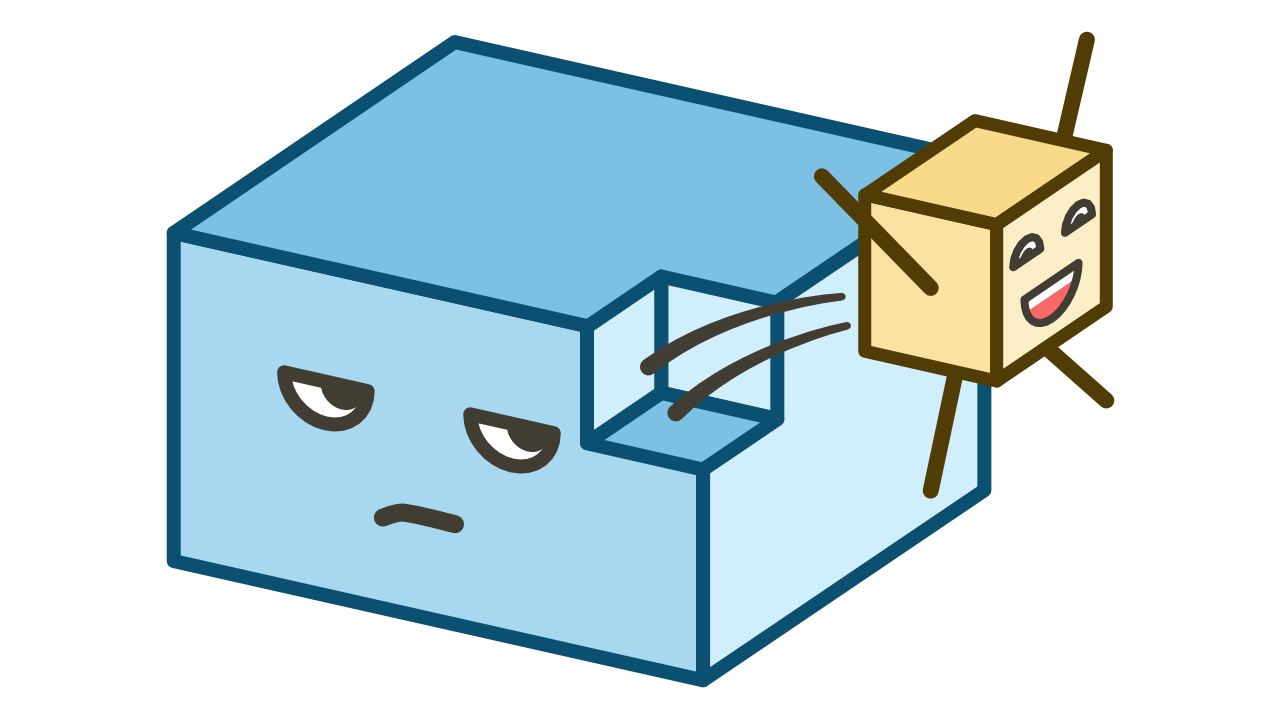
\includegraphics[width=0.4\linewidth]{assets/illustration-monolith-microservice.png}
  \label{fig:illustration-monolith-microservice}
\end{figure}


\section{What is a monolith?}

Before defining a microservice, it is advisable to understand what a monolith is since we are going to use them as a comparison. A monolithic is an "application built as a single unit" ~\cite{microservices.2014}. Enterprise applications are built with a single code base that is maintained in one place by a team or several teams, all working on that one application. Three horizontal layers often separate these applications, the data persistence layer, or database, the server, and the client. The cuts for these layers run along technological boundaries instead of boundaries related to business domains. A business domain is, for example, a part of a software that takes care of user management, another domain may be concerned with all payment-related parts of the application. A layer, however, groups all part of an application that uses the same technology, for example, Java as the server-side language.

The term "monolith" describing an extensive system derives from the Unix community, which uses the term to describe systems that became too big ~\cite{raymond.2003}. When the term is used in literature or conversation, it usually describes a system that has grown very large over time and is very unwieldy for developers to work with. The development of monolith systems tends to be slow, and maintenance is high. Such systems are widespread in the industry and usually so big that several developer teams are needed to keep them running. Because a monolith is a single unit, it is very natural for its programming code to become tightly coupled between its various modules. This has the effect that programmers need more time to understand relationships inside the code than actually writing new code. Developers do not favor large applications of this type.


\section{What is a microservice?}


\begin{itemize}
  \item \done{General definition and how it works}
  \item \done{Get some ideas from the it-innovations article ...}
\end{itemize}

A microservice has four characteristics that set it apart from a monolith.

\subsection{Independently Deployable Services}

Every software is made up of smaller parts, usually called components. The basic concept of Object-Oriented programming, for example, is that all functions and data related to one object, like a product of a store, live in one class. The class houses the data and exposes methods for other parts of the application to interface with its data. The whole application is tied together by function calls that happen inside the memory of a physical machine.

A microservice, on the other hand, is an application that lives on a physically different machine from other services and communicates through mechanisms like an HTTP request. Services don't always have to be on separate machines, but they are always treated like closed systems, and communication happens as if they were on physically separate machines.

Changes in one part of an application that consists of components only take effect when redeploying the whole application. For monoliths, this means that even small changes relative to the entire codebase require a redeploy of the whole system. A system made up of microservices only needs to redeploy the specific service where the change was made. A change in one service may also depend on a change of another service, which means there needs to be some coordination when updating them. However, in general, a microservice is independent of its neighbors and can be deployed and, more importantly, scaled as such.


\subsection{Organized around Business Capabilities}

In his excellent article about microservices ~\cite{microservices.2014} Martin Fowler mentions Conway's Law ~\cite{conway.1968} in regards to large applications. The law states that "any organization that designs a system [...] will inevitably produce a design whose structure is a copy of the organization's communication structure." An organization's structure for software projects often groups different technologies into layers, which leads to different teams skilled for different tasks. An example may be the backend team and the frontend team. Working cross team is usually accompanied by some red tape like budget approvals leading to teams optimizing to solve problems internally. This leads to business logic ending up in places of the system where it shouldn't.

There are many ideas to minimize this effect, a more popular one being Domain-Driven Design ~\cite{evans.2003}. All these approaches, however, call for discipline during development. A microserver, on the other hand, is not organized around technology but a business need. For example, the hands-on part of this paper deals with a service for generating a PDF document. A team working on a microservice, therefore, needs to be cross-functional and therefore avoids organizational barriers.


\subsection{Decentralized Governance}

When splitting an application into multiple services, the developer has the choice of which technology to use. Does he want to build a simple backend API and is comfortable in JavaScript, then he could use Node.js? Is he more familiar with Java, then he could set up a simple Java Spring Framework. Or maybe he needs to use some machine learning model for image processing, in which case Python may be the best choice. Programmers prefer using the right tool for the right job. Monoliths have the inherent limitation that every part of it has to use the same technology. Of course, just because it is possible doesn't mean every service has to use different technology. Often a company is limited by the skillset present among its employees and want's to use this knowledge. Even then, every team has the freedom to define their principles and pick standards best suited for their use-case.

\begin{figure}[ht]
  \centering
  
\includegraphics[width=0.4\linewidth]{assets/illustration-monolith-hammer.png}
  \caption{Not every problem is a nail}
  \label{fig:illustration-monolith-hammer}
\end{figure}

Amazon's "You build it, you run it" methodology is an excellent example of the advantages of decentralized governance ~\cite{amazon.2015}. The idea is that the same team which builds a service is also responsible for running it. According to Stephen Orban, General Manager of an AWS Service, this "forces development teams to think about how their software is going to run in production as they design it." Leading to better software quality and more ownership among the team. Because the developers are ultimately responsible,  they make an effort to avoid bad practices. According to Orban, this even leads to more automation, because developers are inherently lazy and try to avoid repetitive tasks, and more customer satisfaction because the dev team has direct contact with the customer.


\subsection{Decentralized Data Management}

Decentralized data management is likely the single biggest challenge with service-oriented architectures. Monoliths use a single database for the entire application, which makes data management easy. Microservices can also share a single database that would avoid the problem of having to save data in a distributed way or sync data across multiple databases, see figure \ref{fig:decentralised-data}. So why should microservices manage distributed data? The answer is encapsulation, which is a term in computer science, essentially saying that one component should handle all of its concerns internally, and another component should not know about them ~\cite{krivtsov.2019}.

Say there are two microservices, a user service and an order service. Each order is associated with one user who made the order. If both services have their database, then the order service saves the user ID in its database. If a request asks for an order bundled with the user information, then the order service has to make a request of its own to the user service to get the user information in the first place before it can bundle it with its order and send out the answer. If the user service is not available, the order service can not finish the request. Now both services access the same database, and the order service no longer needs the user service because it can merely get into the database and get the user information itself. However, this would mean that the order service knows about the internal affairs of the user service. It knows, for example, how the user table looks like. Now the two services are coupled. If a change is made to the user service, the order service also has to be adjusted. This would effectively undo the benefit of using microservices in the first place and introduce all the challenges of large monoliths into the service-oriented architecture.

\begin{figure}[ht]
  \centering
  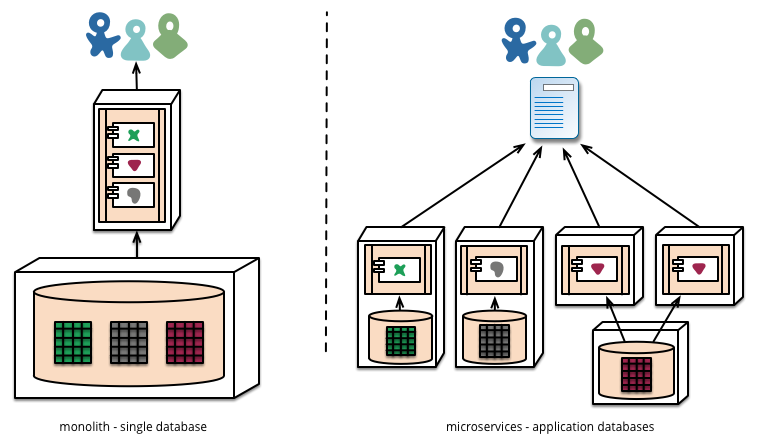
\includegraphics[width=0.7\linewidth]{assets/decentralised-data.png}
  \caption{Data management of monoliths and microservices}
  \source{https://www.martinfowler.com/articles/microservices.html}
  \label{fig:decentralised-data}
\end{figure}

Decentralized data management is the main reason why microservice architectures are not the golden bullet solution. Although the benefits of microservices outweigh monolith architectures in the long run, there is a consensus among developers that it is better to start with a monolith. Then refactor to microservices later "if you really need them in the future." ~\cite{krivtsov.2019}


\section{Why are microservices currently interesting?}

\begin{itemize}
  \item \todo{(Why)}
  \item \todo{Application development until now with monoliths \& waterfall}
  \item \todo{Avarage life and maintenance effort of a big application}
  \item \todo{Rise of Agile, the Cloud and quick deployment cycles}
\end{itemize}


\section{Which problem does a microservice solve?}
\label{sec:theory:what-problem}

\begin{itemize}
  \item \todo{(Why)}
  \item \todo{Why is a microservice better than a monolith?}
  \item \todo{Advantages \& Disadvantages of microservices}
  \item \todo{Work/Effort of microservice compared to monolith}
\end{itemize}


\section{When does a microservice make sense?}

\begin{itemize}
  \item \todo{(Why)}
  \item \todo{What type of application are microservices best suited for? (Scallable, defined scope)}
  \item \todo{Good size of a team for a microservice}
  \item \todo{When not to use distributed service architecture}
\end{itemize}


\section{How to extract a microservice?}

\begin{itemize}
  \item \todo{(How)}
  \item \todo{How to make a cut in a big application (monolith)}
\end{itemize}


\section{Challenges of implementing a microservice}

\begin{itemize}
  \item \todo{Complexity of ecosystem}
  \item \todo{Design challange because often monolith software is old and overcomplicated. This complication should be simplified in the new microservice.}
\end{itemize}
